\chapter{Algoritmos de clustering con restricciones}\label{ch:Algoritmos de clustering con restricciones}

Una vez introducido el problema del clustering con restricciones, pasamos a profundizar en los métodos para su aplicación. La siguiente sección presenta 5 algoritmos de clustering con restricciones, cuyos resultados serán expuestos más tarde, en la sección XX (referencia a la experimentación).

\section{Formalización del problema}

Definido ya el problema del clustering con restricciones en la sección \ref{ch:Clustering con restricciones}, especificamos la manera de notar sus elementos, de forma que sea sencillo referirse a ellos.

\begin{itemize}
	
	\item Notaremos con $X$ a la matriz de $n\times p$ que contiene el conjunto de datos de entrada.
	
	\item Notaremos con $x_i \;\; t.q. \;\; i \in \{1, \cdots, n\}$ a cada instancia de $X$, por lo que $x_i$ es un vector en el espacio $\mathbb{R}^p$ ($x_i \in \mathbb{R}^p$).
	
	\item Notaremos con $R$ al conjunto de restricciones, tanto las de tipo \acs{ML} como las \acs{CL}, es decir $R = ML \cup CL$. 
	
	\item Notaremos con $k$ el número de clusters de la partición resultante.
	
	\item Notaremos con $C$ el conjunto de clusters, y con $c_i \; t.q. \; i \in \{1, \cdots, k\}$ a cada uno de ellos, por tanto $C = \{c_i, \cdots, c_k\}$.
	
	\item Notaremos con $V$ la matriz de $k\times p$ que almacena el conjunto de centroides asociados a los clusters, de manera que $v_i \in \mathbb{R}^p$ corresponde al cluster $c_i$.
	
\end{itemize}

Cabe destacar que los elementos y parámetros particulares de cada algoritmo serán definidos en la sección correspondiente al mismo, así como que no todos los elementos expuestos anteriormente son comunes a todos los algoritmos; si bien si que lo son a la mayoría.

\section{COP-k-means (Constrained k-means)}

El algoritmo k-medias (\textit{k-means}) es uno de los más básicos para aplicar clustering. Así, el algoritmo COP-k-medias (\textit{COP-k-means}) es la adaptación inmediata de k-medias al clustering con restricciones. Para realizar un estudio detallado sobre el mismo tomaremos como base el trabajo de Wagstaff et al. (2001) \cite{Wagstaff:2001b}.

El cambio más notable que supone COP-k-medias respecto al tradicional k-medias, consiste en modificar la regla de asignación de instancias a clusters de este último, para comprobar que dicha asignación no viola ninguna restricción. De esta manera, en cada iteración se intenta asignar cada instancia $x_i$ al cluster más cercano $c_j$. Ésta asignación solo se llevará a cabo si, como hemos dicho, no se viola ninguna restricción. Si existe una instancia $x_{ML}$ que debe ser asignada al mismo cluster que $x_i$, pero ya ha sido incluida en otro cluster, o existe una instancia $x_{CL}$ en $c_j$ que no puede ser agrupada junto a $x_i$, entonces $x_i$ no puede ser asignado a $c_j$. El proceso continua hasta encontrar una asignación legal para $x_i$, en caso de que no se encuentre se devuelve la partición vacía como resultado. Así el algoritmo da como resultado una partición de $X$ que cumple necesariamente todas las restricciones especificadas en $R$. El algoritmo \ref{alg:ckm} corresponde al pseudocódigo asociado a COP-k-medias \cite{Wagstaff:2001b}:


\begin{algorithm}
	
	\BlankLine
	\KwIn{Conjunto de datos $X$, conjunto de restricciones $R$}
	\KwOut{Partición $P$ del conjunto de datos $X$}
	\BlankLine
	\textbf{función} COP-K-means($X$, $R$) \Begin{
		\BlankLine
		1. Sean $C = \{c_1\cdots c_k\}$ los clusters iniciales\\
		2. Asignar cada instancia $x_i \in X$, al centroide más cercano $c_j$ tal que ViolaRestriccion($x_i$, $c_j$, $R$) = falso. Si no existe $c \in C \;\;\; t.q.$ ViolaRestriccion($x_i$, $c_j$, $R$) = falso, \KwRet $\emptyset$.\\
		3. Para cada cluster $c_i$, actualizar su centroide realizando un promedio de todas las instancias $x_i$ asignadas a él.\\
		4. Iterar entre (1.) y (2.) hasta converger.\\
		5. \KwRet $C$
		\BlankLine
	}
	\BlankLine
	\KwIn{Instancia $x$, cluster $c$, conjunto de restricciones $R$}
	\BlankLine
	\textbf{función} ViolaRestriccion($x$, $c$, $R$) \Begin{
		\BlankLine
		1. Para cada $(x, x_{ML}) \in ML$, si $x_{ML} \notin R$ \KwRet \textbf{true}.\\
		2. Para cada $(x, x_{CL}) \in CL$, si $x_{CL} \notin R$ \KwRet \textbf{true}.\\
		3. En otro caso, \KwRet \textbf{false}.
		\BlankLine
	}
	
	\caption{COP-k-means}\label{alg:ckm}
\end{algorithm}

Existen multitud de criterios de convergencia estandarizados, aunque es común emplear uno adaptado al problema particular que queramos solucionar. El más extendido consiste en calcular la diferencia de la posición de los centroides entre dos iteraciones sucesivas, de forma que cuando esta sea menor que un umbral dado detenemos el proceso de iteración.

\clearpage

\section{CEKM (Constrained Evidential k-means)}

Tal y como indican Violaine el al. (2012) \cite{CECM:2012}, cuyo trabajo es el fundamento de la siguiente sección, para comprender el algoritmo  \acf{CEKM}, primero es necesario realizar una introducción al algoritmo k-medias difuso (\textit{fuzzy k-means}). En él, cada instancia puede pertenecer a uno o más clusters, con diferentes grados de pertenencia. La matriz que almacena esta información, es decir, la partición difusa, se nota con $U$, y se calcula minimizando la siguiente función:

\begin{equation}
\sum_{j=1}^{k} u_{ij} \;\; t.q. \;\; u_{ij} \in [0,1] \forall i,j
\label{eqn2}
\end{equation}

Donde $u_{ij}$ representa el grado de pertenencia de la instancia $i$ al cluster $j$, y $k$ es el número de clusters. Sin embargo, este método puede producir resultados contraintuitivos cuando los datos a los que se aplica son ruidosos o presentan instancias aisladas (\textit{outliers}).

El clustering evidencial (\textit{evidential clustering}) da solución a los problemas que presenta el algoritmo k-medias difuso, introduciendo el concepto de partición de creencia (\textit{credal partition}), que extiende los conceptos existentes de particiones fuertes, difusas y probabilísticas. De esta forma, en una partición de creencia, se asigna a cada instancia una masa de creencia (\textit{mass of belief}) no solo para un único cluster, sino para cualquier conjunto de los mismos. El método \acs{CEKM} combina las ventajas del uso de las restricciones con las del uso de funciones de creencia.

\subsection{Funciones de creencia}

La teoría de la evidencia de Dempster-Shafer ofrece un marco teórico para trabajar con información parcial y no completamente fiable, tomamos de ella los conceptos relativos a las funciones de creencia.

Consideremos la variable $c$ que toma valores en el conjunto finito $C = \{c_1 \cdots c_k \}$. El conocimiento parcial sujeto al valor real que adopta $c$ puede ser representado mediante una función de masa $m$, que es una aplicación de $C$ al intervalo $[0,1]$:

\begin{equation}
\sum_{A \subseteq C} m(A) = 1
\label{eqn3}
\end{equation}

A los subconjuntos $A$ de $C$ que cumplen que $m(A) > 0$ se los denomina conjuntos focales (\textit{focal sets}) de $m$. El valor del conjunto focal $m(A)$ se interpreta como la fracción de una unidad de masa de creencia que está asignada a $A$ y que no puede ser asignada a ningún otro subcojunto de $A$. Si el único conjunto focal es $C$, nos encontramos en el caso de completa ignorancia sobre los datos. Por el contrario, si la masa de creencia se asigna a un único elemento de $C$, estaríamos en el caso de certeza absoluta.

Se dice que una función de masa $m$ está normalizada si $m(\emptyset) = 0$. Sin embargo, bajo la hipótesis de mundo abierto, una función de masa en la que $m(\emptyset) > 0$ se interpreta como la cantidad de creencia que se le asigna a la hipótesis de que el verdadero valor de $c$ puede no encontrarse en $C$.

Dada una función de masa $m$, podemos definir una función de plausibilidad $pl:2^C \rightarrow [0,1]$ y una función de creencia $bel: 2^C \rightarrow [0,1]$ de la siguiente manera:

\begin{equation}
pl(A) = \sum_{B \cap A \neq \emptyset} m(B) \;\;\; \forall A \subseteq C
\label{eqn4}
\end{equation}

y 

\begin{equation}
bel(A) = \sum_{B \subseteq A, B \neq \emptyset} m(B) \;\;\; \forall A \subseteq C
\label{eqn5}
\end{equation}

De esta manera, las funciones $pl$ y $bel$ están relacionadas como sigue:

\begin{equation}
pl(A) = 1 - m(\emptyset) - bel(\bar{A})
\label{eqn6}
\end{equation}

Donde $\bar{A}$ representa el complemento de $A$.  La cantidad $bel(A)$ se interpreta como el grado de creencia en $A$, tomando en consideración la masa de creencia asignada a $A$ y a los subconjuntos no vacíos de $A$. Por el contrario, $pl(A)$ mide hasta que punto es erróneo no creer en $\bar{A}$.

Con el objetivo de tomar decisiones en base al valor de $c$, es posible transformar la función de masa en una distribución de probabilidad pignística, definida, para una función de masa normalizada, como:

\begin{equation}
BetP(c) = \sum_{c \in A} \frac{m(A)}{|A|} \;\;\; \forall c \in C
\label{eqn7}
\end{equation}

\subsection{FKM (fuzzy k-means) y sus variantes}

Cada cluster $c_j \in C$ con $j \in \{1,\cdots,k\}$ esta representado por un vector $v_j \in \mathbb{R}^p$, es decir, un centroide. Además, definimos $V$ como la matriz compuesta por todos los centroides, y $U = (u_{ij})$ como la partición difusa que contiene los grados de pertenencia de cada instancia de $X$ a cada cluster. El algoritmo k-medias difuso calcula las matrices $U$ y $V$ de manera que minimiza (sujeto a las ecuaciones \ref{eqn2} y \ref{eqn3}) la siguiente función:

\begin{equation}
J_{FKM}(U,V) = \sum_{i=1}^{n}\sum_{j=i}^{k} u_{ij}^\beta d_{ij}^2
\label{eqn8}
\end{equation}

Donde $d_{ij}$ representa la distancia euclidea entre el objeto $x_i$ y el centroide $v_j$, y donde $\beta > 1$ es el exponente que controla el grado de difusión de la partición. La función objetivo se minimiza mediante un algoritmo iterativo que optimiza los centroides y los grados de pertenencia de manera alterna. El algoritmo empieza con una asignación inicial sobre la que realiza modificaciones hasta que converge.

Para detectar datos ruidosos u outliers empleamos el algoritmo \acs{NC} \textit{Noise-Clustering}. Este método consiste en añadir a los $k$ clusters iniciales uno adicional llamado ``cluster ruidoso'', asociado a una distancia fija $\rho$ respecto a todos los objetos. El parámetro $\rho$ controla la cantidad de datos que serán considerados como outliers. La pertenencia $u_{i*}$ de un objeto $i$ al cluster ruidoso se calcula como:

\begin{equation}
u_{i*} = 1 - \sum_{j=1}^{k} u_{i,j} \;\;\; i = {1,\cdots,n}
\label{eqn9}
\end{equation}

Por tanto, la función objetivo que minimiza el algoritmo \acs{NC} no es más que una combinación del cálculo de pertenencia de objetos al cluster ruidoso y la que minimizaba el algoritmo k-medias difuso:

\begin{equation}
J_{NC}(U,V) = \sum_{i=1}^{n}\sum_{j=i}^{k} u_{ij}^\beta d_{ij}^2 + \sum_{i=1}^{k} \rho^2 u_{i*}^\beta
\label{eqn10}
\end{equation}

\subsection{El algoritmo EKM (Evidential k-means)}

Es posible obtener una versión credibilística del algoritmo \acs{NC} reemplazando la matriz asociada a la partición difusa $U$ con una partición de creencia, que notaremos con $M$. En este contexto, el conocimiento parcial asociado a la pertenencia de un objeto a una clase, viene representado por una función de masa aplicada al conjunto $C$ de posibles clases. Por tanto, la masa de creencia puede ser asignada a cualquier subconjunto $A$ de $C$, y no sólo a elementos únicos de $C$. Este esquema hace posible modelar una amplia variedad de circunstancias, que van de la completa ignorancia sobre el conjunto de datos hasta la completa certeza sobre el mismo.

Para ilustrar estas ideas se propone el siguiente ejemplo: consideramos un conjunto de cuatro objetos que deben ser clasificados en dos clases. El cuadro \ref{tab:tabla2} contiene la partición de creencia asociada a estos datos. La clase del primer objeto es conocida con certeza, ya que su masa de creencia esta asignada a un solo elemento de $C$. Por el contrario la clase del segundo objeto es completamente desconocida. La masa de creencia del tercer objeto esta repartida entre dos elementos de $C$, por tanto tenemos conocimiento probabilístico sobre la clase a la que pertenece. El último objeto representa un outlier, ya que su masa de creencia está asignada al conjunto vacío.

\begin{table}[h]
	\centering
	\setlength{\arrayrulewidth}{1mm}
	\setlength{\tabcolsep}{10pt}
	\renewcommand{\arraystretch}{1}
	
	\rowcolors{2}{gray!25}{white}
	\begin{tabular}{ >{\centering\arraybackslash}m{1cm}  >{\centering\arraybackslash}m{1cm}>{\centering\arraybackslash}m{1cm}>{\centering\arraybackslash}m{1cm}>{\centering\arraybackslash}m{1cm}}
		\hline
		\rowcolor{black}
		\multicolumn{5}{c}{\bf \color{white}{Ejemplo de partición de creencia}}\\
		\hline
		\rowcolor{gray!50}
		\textbf{$A$} & \textbf{$m_1(A)$} & \textbf{$m_2(A)$} & \textbf{$m_3(A)$} & \textbf{$m_4(A)$} \\
		$\emptyset$ & 0 & 0 & 0 & 1 \\
		$\{c_1\}$ & 1 & 0 & 0.3 & 0 \\
		$\{c_2\}$ & 0 & 0 & 0.7 & 0 \\
		$C$ & 0 & 1 & 0 & 0 \\
		\hline
		
	\end{tabular}
	\caption[Ejemplo de partición de creencia]{Ejemplo de partición de creencia \cite{CECM:2012}}
	\label{tab:tabla2}
\end{table}

\acf{EKM} es uno de los algoritmos que opera con una partición de creencia obtenida en base a los datos. Si tomamos $m_{ij}$ como el grado de creencia de que el objeto $x_i$ pertenece al subconjunto $A_j \subseteq C$, obtener una partición de creencia implica determinar, para cada $x_i$, las cantidades $m_{ij} = m_i(A_j)\;\; \forall A_j \neq \emptyset, A_j \subseteq C$. De esta manera, cuando la distancia $d_{ij}$ entre $x_i$ y $A_j$ es alta (baja), $m_{ij}$ será un valor bajo (alto).

Tal y como sucedía en el algoritmo k-medias difuso, cada clase $c_l$ está representada por un centroide $v_l \in \mathbb{R}^p$. Entonces, para cada subconjunto $A_j$ de $C$ distinto de $\emptyset$ se calcula su centroide $\bar{v}_j$ como el baricentro de los centros asociados a las clases presentes en $A_j$:

\begin{equation}
\bar{v}_j = \frac{1}{|A_j|} \sum_{l=1}^{k} S_{lj} v_l
\label{eqn11}
\end{equation}

donde el valor $S_{lj}$ viene definido por:

\begin{equation}
S_{lj} = \begin{cases}
1 \;\;\; \textbf{si} \;\;\; c_l \in A_j\\
0 \;\;\; \textbf{otro caso}
\end{cases}
\label{eqn12}
\end{equation}

La distancia $d_{ij}$ entre la instancia $x_i$ y el conjunto focal $A_j$ se calcula como:

\begin{equation}
d_{ij} = ||x_i - \bar{v}_j||
\label{eqn13}
\end{equation}

Entonces, el algoritmo \acs{EKM} calcula las matrices $M$ y $V$ tratando de minimizar un criterio similar al del algoritmo \acs{NC}:

\begin{equation}
J_{EKM}(M,V) = \frac{1}{2^cn} \sum_{i=1}^{n}\sum_{A_j \neq \emptyset} |A_j|^\alpha m_{ij}^\beta d_{ij}^2 + \sum_{i=1}^{n} \rho^2 m_{i\emptyset}^\beta
\label{eqn14}
\end{equation}

sujeto a las restricciones $m_{ij} \ge 0 \;\; \forall i,j$, y $m_{i\emptyset} \ge 0 \;\; \forall i$, y:

\begin{equation}
\sum_{j/A_j \subseteq C, A_j \neq \emptyset} m_{ij} + m_{i\emptyset} = 1 \;\;\; \forall i = 1,n
\label{eqn15}
\end{equation}

Donde $m_{i\emptyset}$ denota la cantidad de masa de creencia de la instancia $x_i$ asignada al conjunto vacío. El parámetro $\rho$ representa la distancia de cualquier objeto al conjunto vació, y el parámetro $\alpha$ se introduce para controlar la penalización por asignar objetos a conjuntos con alta cardinalidad.

Gracias a la restricción expuesta en la ecuación \ref{eqn15}, podemos obtener equivalencia entre los algoritmos \acs{NC} y \acs{EKM}. El algoritmo \acs{EKM} asigna una gran masa de creencia al conjunto vacío para un objeto dado cuando éste se encuentra lejos de todos los subconjuntos $A_j$.

Como en \acs{FKM} y \acs{NC}, la partición de creencia se calcula aplicando un proceso de optimización iterativo, que actualiza las masas  y los centroides de forma alterna. La regla de optimización de $M$ es muy similar a su homóloga en \acs{NC}, excepto por el número de valores $m_{ij}$ a calcular, que en este caso es $2^c$, en lugar de los $k + 1$ grados de pertenencia que eran necesarios en \acs{NC}. De esta manera, la función de masa queda definida como:

 \begin{equation}
m_{ij} = \frac{|A_j|^{-\alpha/(\beta-1)} d_{ij}^{-2/(\beta-1)}}{\sum_{A_l \ne \emptyset}|A_l|^{-\alpha/(\beta-1)} d_{ij}^{-2/(\beta-1)} + \rho^{-2/(\beta-1)}}
 \label{eqn16}
 \end{equation}
 
 y
 
\begin{equation}
m_{i\emptyset} = 1 - \sum_{A_j \ne \emptyset}m_{ij} \;\;\; i = 1,n
\label{eqn17}
\end{equation}

Por otra parte, la regla de actualización de los centroides resulta un poco más compleja. Requiere resolver un sistema de ecuaciones lineal en cada paso del proceso, en el que cada columna de $V$ es la solución para un sistema lineal de $k$ ecuaciones y $k$ incógnitas. Tomamos $B$ como la matriz de tamaño $(k \times p)$ definida por:

\begin{equation}
B_{lq} = \sum_{i=1}^{n} X_{iq} \sum_{A_j \ni c_l} |A_j|^{\alpha-1} m_{ij}^\beta \;\;\; l = 1,k \;\;\; q =1,p
\label{eqn18}
\end{equation}

y la matriz $H$ de tamaño $(k \times k)$ como:

\begin{equation}
H_{lk} = \sum_{i} \sum_{A_j \supseteq \{c_t,c_l\}} |A_j|^{\alpha - 2} m_{ij}^\beta \;\;\; t,l = 1,k
\label{eqn20}
\end{equation}

de forma que $V$ es la solución del sistema de ecuaciones lineal $H\times V = B$, que puede ser resuelto mediante técnicas estándar.

\subsection{Incorporación de restricciones a EKM}

Una vez definidos los elementos que conforman el algoritmo \acs{EKM}, debemos incorporar las restricciones a nivel de instancia al marco de las funciones de creencia, para integrarlas en el cálculo de la partición de creencia.

Siendo $x_i$ y $x_j$ dos instancias, podemos calcular la función de masa conjunta en el producto cartesiano $C \times C = C^2$ conociendo sus funciones de masa particulares $m_i$ y $m_j$:

\begin{equation}
m_{i \times j}(A \times B) = m_i(A)m_j(B) \;\;\; A,B \subseteq C, A \neq \emptyset, B \neq \emptyset
\label{eqn21}
\end{equation}

\begin{equation}
m_{i \times j}(\emptyset) = m_i(\emptyset) + m_j(\emptyset) - m_i(\emptyset)m_j(\emptyset)
\label{eqn22}
\end{equation}

Conociendo $ m_{i \times j} $ es posible calcular la plausibilidad asociada a que los objetos $x_i$ y $x_j$ pertenezcan a la misma clase que, en el espacio $C^2$, corresponde al subconjunto $\theta = \{(c_1, c_1), (c_2, c_2), \cdots, (c_k, c_k)\}$. El caso contrario corresponde al complemento de $\theta$, es decir, $\bar{\theta}$

\begin{equation}
pl_{i\times j}(\theta) = \sum_{A \cap B \ne \emptyset}m_i(A)m_j(B)
\label{eqn23}
\end{equation}
\begin{equation}
pl_{i\times j}(\bar{\theta}) = 1 - m_{i\times j}(\emptyset) - \sum_{l=1}^{k} m_i(\{c_l\})m_j(\{c_l\})
\label{eqn24}
\end{equation}

\subsection{Función objetivo de CEKM}

Asumimos ahora que la partición de creencia es desconocida, y que disponemos del conjunto de restricciones. En tal caso será necesario buscar una partición de creencia que considere las similitudes y diferencias obtenidas en base a los datos, así como las restricciones. Para ello debemos buscar que $pl_{i\times j} (\theta)$ sea tan bajo como sea posible si $(x_i, x_i) \in CL$, así como que $pl_{i\times j} (\bar{\theta})$ lo sea si $(x_i, x_i) \in ML$. A tal fin, integramos una penalización en el criterio de optimización de \acs{EKM} de la siguiente manera:

\begin{equation}
J_{CONST} = \frac{1}{|R|} \left[\sum_{(x_i,x_j) \in ML} pl_{i\times j} (\bar{\theta})\;\; + \sum_{(x_i,x_j) \in CL} pl_{i\times j} (\theta)\right]
\label{eqn25}
\end{equation}

De esta forma, la función objetivo a minimizar pasa a ser:

\begin{equation}
J_{CEKM}(M,V) = (1- \xi)J_{EKM}(M,V) + \xi J_{CONST}
\label{eqn26}
\end{equation}

donde el parámetro $\xi \in [0,1]$ se utiliza para controlar el compromiso entre las restricciones y el modelo geométrico asociado a la métrica de distancia.

\subsection{Proceso de optimización de CEKM}

De igual forma que en \acs{FKM}, \acs{NC} y \acs{EKM}, el modelo de optimización de \acs{CEKM} consiste en actualizar $M$ y $V$ de forma alterna. Cabe destacar que el termino de penalización añadido a \acs{CEKM} no depende de los centroides de los clusters, y por tanto se pueden aplicar el mismo modelo de actualización que en \acs{EKM} (ecuaciones \ref{eqn18} y \ref{eqn20}). Generalmente, el problema es mucho más complejo para las masas de creencia. Sin embargo fijando $\beta = 2$, la función objetivo \ref{eqn26} pasa a ser cuadrática respecto a $m_{ij}$. Con esto, y como las restricciones son lineales, se pueden emplear algoritmos de programación cuadrática para resolver el problema de la actualización de las masas de creencia. El proceso de cálculo asociado a \acs{CEKM} queda resumido en el algoritmo \ref{alg:cecm}. 


\begin{algorithm}
	
	\BlankLine
	\KwIn{Conjunto de datos $X$, conjunto de restricciones $R$, número de clusters resultantes $k$}
	\KwOut{Partición de creencia $M$, centroides $V$}
	\BlankLine
	\textbf{función} CEKM($X$, $R$, $k$) \Begin{
		\BlankLine
		1. Inicialización de $V$\\
		2. Actualizar las masas ($M$) resolviendo el problema de programación cuadrática definido por \ref{eqn26} sujeto a \ref{eqn15}\\
		3. Actualizar los centroides ($V$) resolviendo el sistema de ecuaciones lineal definido por \ref{eqn18} y \ref{eqn20} con $\beta = 2$\\
		4. Iterar entre (2.) y (3.) hasta que no haya cambios significativos en $V$.\\
		5. \KwRet $M$, $V$
		\BlankLine
	}
	\caption{\acs{CEKM}}
	\label{alg:cecm}
\end{algorithm}

En la mayoría de las ocasiones se requiere como resultado de un algoritmo de clustering una partición fuerte del conjunto de datos, y no una partición de creencia. Podemos obtener una partición difusa calculando la probabilidad pignística $BetP_i(\{c_j\})$ en base a cada función de masa $m_i$ aplicando la ecuación \ref{eqn7}, e interpretar este valor como el grado de pertenencia del objeto $i$ al cluster $j$. Una vez obtenida la partición difusa podemos procesarla como precise el problema para obtener la partición fuerte. La manera más común de hacerlo es asignar cada instancia al cluster para el que presente un mayor grado de pertenencia.

Otra manera de extraer información de la partición de creencia es asignar cada objeto al subconjunto de clases que contengan un mayor porcentaje de su masa de creencia. De esta forma obtenemos una partición de creencia fuerte de, como mucho, $2^k$ clusters. A partir de esta partición es posible discernir que objetos deben ser asignados a un único cluster sin ambigüedad, además de detectar aquellos que se encuentran en la frontera de dos o más clusters, que a menudo suelen ser relevantes.

\section{Linear Constrained Vector Quantization Error (LCVQE)}

Tomando como base el trabajo de Pelleg y Dorit \cite{LCVQE:2007}, es necesario realizar una introducción al algoritmo \acf{CVQE} antes de detallar el algoritmo \acs{LCVQE}, puesto que este último consiste en una modificación sobre el primero para mejorar, principalmente, su orden de complejidad.

\subsection{El algoritmo CVQE}

El algoritmo CVQE consiste en una generalización del algoritmo k-medias para incluir las restricciones. En el algoritmo k-medias cada centroide $v_i$ se actualiza en cada iteración siguiendo la regla:

\begin{equation}
v_i = \frac{1}{|c_i|} \sum_{x_i \in c_i} x_i
\label{eqn27}
\end{equation}

Que no es más que un promedio de todas las instancias asignadas al cluster asociado al centroide $v_i$. Tras la actualización, se recalculan las asignaciones para que cada instancia este asociada al cluster más cercano, lo que deriva en una regla que minimiza la función \acf{VQE}:

\begin{equation}
VQE = \frac{1}{2} \sum_{j = i}^{k} \sum_{x_i \in c_i} (v_j - x_i)^2
\label{eqn28}
\end{equation}

\acs{CVQE} modifica la función \acs{VQE} añadiendo de la misma un término de penalización que considera las restricciones incumplidas por una asignación de instancias a clusters dada. Por simplicidad, notaremos el cardinal de $ML$ con $ml$, así como el de $CL$ con $cl$, y definiremos el conjunto de restricciones $R$ como una lista de parejas de instancias: 

\begin{equation}
\{(x_1(i), x_2(i))\}_{i=1}^{ml+cl}
\label{eqn29}
\end{equation}

Además definimos $M$ como la función que, dada una instancia, devuelve el índice del cluster al que está asignada: $M = \{j | x \in c_j\}$, así como las funciones $g(i) = M(x_1(i))$ y $g^\prime(i) = M(x_r(i))$. Por otra parte, definimos $h(i)$ como la función que devuelve el centroide más cercano al centroide $v_i$. Finalmente definimos $vl(i)$ de manera que indica si las restricción i-ésima ha sido violada, por tanto, para $i = 1, \cdots , ml \;\; vl(i) = 1 \leftrightarrow g(i) \neq g^\prime(i)$, de forma similar $i = ml + 1, \cdots , ml + cl \;\; vl(i) = 1 \leftrightarrow g(i) = g^\prime(i)$. Definidas estas funciones, la regla de actualización de \acs{CVQE} es:

\begin{equation}
v_j = \frac{1}{N_j} \left[ \sum_{x_i \in C_i}x_i + 
\sum_{l=1,g(l) = j}^{ml} vl(l) v_{g^\prime(l)} + 
\sum_{l=ml + 1,g(l) = j}^{ml + cl} vl(l) v_{h(g^\prime(l))}
\right]
\label{eqn30}
\end{equation}

donde $N_j$ viene definido por: 

\begin{equation}
N_j = |c_j| + \sum_{l=1,g(l) = j}^{ml + cl} vl(l)
\label{eqn31}
\end{equation}

De manera intuitiva, para las restricciones $ML$ incumplidas, uno de los dos centroides afectados se mueve hacia el otro, mientras que para las $CL$ incumplidas se mueve uno de las instancias hacia el siguiente centroide más cercano a su cluster. De forma similar a k-medias, cada instancia se reasigna después de cada iteración para minimizar la función de error $CVQE = \sum_{j=i}^{k} CVQE_j$, donde $CVQE_j$ es:

\begin{equation}
CVQE_j = \frac{1}{2} \sum_{x_i \in C_j} T_{j,1} + 
\frac{1}{2} \sum_{l=1,g(l) = j}^{ml} T_{j,2} + 
\frac{1}{2} \sum_{l=ml + 1,g(l) = j}^{ml + cl} T_{j,3}
\label{eqn32}
\end{equation}

donde los términos $T_{j,1}$, $T_{j,2}$ y $T_{j,3}$ vienen definidos como: 

\begin{equation}
T_{j,1} = (v_j - x_i)^2
\label{eqn33}
\end{equation}

\begin{equation}
T_{j,2} = \left[ (v_j - v_{g^\prime(l)})^2 \cdot vl(l) \right]
\label{eqn34}
\end{equation}

\begin{equation}
T_{j,3} = \left[ (v_j - v_{h(g^\prime(l))})^2 \cdot vl(l) \right]
\label{eqn35}
\end{equation}

Cabe destacar que, al contrario de lo que sucede en k-means, en \acs{CVQE}, un cluster $c_i$ puede contener instancias para las que el centroide $v_j$ no es el más cercano a ella.

En cada paso, el algoritmo \acs{CVQE} asigna asigna cada par de instancias implicadas en una restricción de manera que se minimiza la función $CVQE$.

A continuación se exponen algunas de las características del algoritmo \acs{CVQE} que resultan relevantes para la compresión de \acs{LCVQE}.

En primer lugar, el orden en el que se especifican las instancias implicadas en las restricciones es relevante. Consideremos una restricción formada por las instancias $(x_i(l), x_2(l))$, de forma que $x_1(l) \in c_{g(l)}$, y $x_2(l) \in c_{g^\prime(l)}$. Solo $c_{g(l)}$ se ve afectado por violar la restricción, mientras que sobre $c_{g^\prime(l)}$ no se aplica ninguna cambio. Esta regla se cumple tanto para las restricciones \acf{ML} como para las \acf{CL}.

El segundo lugar, determinar la asignación que minimiza la función de error requiere $\mathcal{O}(k^2)$ cálculos para cada restricción. Por tanto, el método puede resultar computacionalmente pesado para grandes conjuntos de restricciones o clusters. Además, no es posible descartar ninguna opción de los cálculos a parte de las triviales. Para ejemplificar esto consideramos la figura \ref{fig:figure19}. En ella, el par $(x,y)$ es una restricción \acs{ML}, y los centroides existentes son $\{v_1,\cdots,v_6\}$. Dependiendo de los valores $R$, $\delta$ y $\epsilon$ las instancias pueden ser asignadas a los centroides $(v_1, v_2)$, $(v_3, v_4)$, $(v_5, v_6)$. Por tanto, las $k^2$ opciones deben ser consideradas para cada restricción al decidir una asignación.

\begin{figure}[!h]
	\centering
	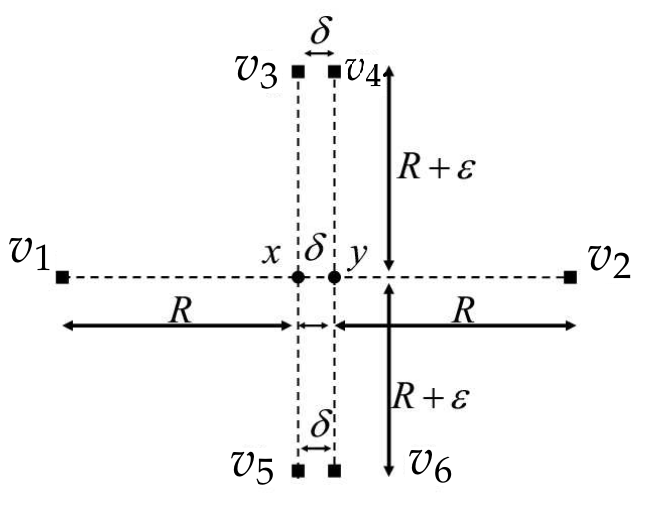
\includegraphics[scale=0.3]{imagenes/c4/Fig1}
	\caption[Ejemplo de CVQE.]{Ejemplo de CVQE. \cite{LCVQE:2007}}\label{fig:figure19}
\end{figure}

La última observación esta relacionada con el hecho de que la penalización por violar restricciones depende de la distancia entre los cetroides implicados en ella, pero no de la distancia entre las instancias. Para mostrar el problema que esto supone tomamos la imagen \ref{fig:figure20}. En ella se presentan dos problemas de clustering, para ambos, los centroides existentes son $v_1$ y $v_2$, mientras que un problema incluye la restricción $ML(x_1, y)$ y el otro $ML(x_2, y)$.


\begin{figure}[!h]
	\centering
	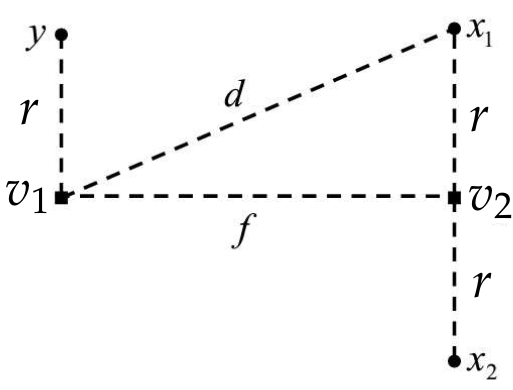
\includegraphics[scale=0.3]{imagenes/c4/Fig2}
	\caption[Ejemplo de CVQE.]{Ejemplo de CVQE. \cite{LCVQE:2007}}\label{fig:figure20}
\end{figure}

El cuadro  recoge las asignaciones posibles en cada caso y el valor de la función $CVQE$. Vemos que, independientemente del valor de $d$ y $f$, ambos problemas tiene la misma solución, mientras que intuitivamente diríamos que violar la restricción $ML(x_1, y)$ debería acarrear una penalización mayor que violar $ML(x_2, y)$. Es más, en ambos casos la acción que aplica \acs{CVQE} es la misma, mover $v_1$ hacia $v_2$ en la recta que los une.

\begin{table}[!h]
	\centering
	\setlength{\arrayrulewidth}{1mm}
	\setlength{\tabcolsep}{10pt}
	\renewcommand{\arraystretch}{0.9}
	
	\rowcolors{2}{gray!25}{white}
	\begin{tabular}{ >{\centering\arraybackslash}m{2cm}  >{\centering\arraybackslash}m{2.5cm}>{\centering\arraybackslash}m{2cm}>{\centering\arraybackslash}m{2cm}}
		\hline
		\rowcolor{black}
		\multicolumn{4}{c}{\bf \color{white}{Valores de CVQE}}\\
		\hline
		\rowcolor{gray!50}
		\textbf{Restricción} & \textbf{$y \in c_1, x_i \in c_2$} & \textbf{$x_i,y \in c_1$} & \textbf{$x_i,y \in c_2$}  \\
		$ML(x_1, y)$ & $R^2 + R^2 + f^2$ & $R^2 + f^2 $ & $R^2 + d^2 $  \\
		$ML(x_2, y)$ & $R^2 + R^2 + f^2$ & $R^2 + f^2 $ & $R^2 + d^2 $  \\
		\hline
		
	\end{tabular}
	\caption[Ejemplo de partición de creencia]{Ejemplo de partición de creencia \cite{CECM:2012}}
	\label{tab:tabla3}
\end{table}

\subsection{El algoritmo LCVQE}












%\section{Relational Dirichlet Process - Means (RDP - Means)}


%\section{Two View Clustering (TV-Clust)}



